\section{Control}
So far we have analyzed our system as a continuous system.
However, we are using the Raspberry Pi to control the robot, so we will
be using digital control. It's a branch of control theory that uses
digital computers to act as system controllers.

In order to sample the position and the speed we use the rotatory encoders.
They count the number of flags so there is a constant to convert them into radians.

All our digital control was made in periodical loops. To get the speed we
divided the incremental position by the period of the loop. All the controllers
are PID controllers, each of time with different inputs, constants and outputs.

A PID controller continuously calculates an error value $e(t)$ as the difference between
a desired set point and a measured process variable and applies a
correction based on proportional, integral, and derivative terms
(denoted $K_p$, $K_i$, and $K_d$ respectively).

To adjust the controller constants in all cases we did the following way:

\begin{enumerate}
    \item Set all gains to zero.
    \item Increase the $K_p$ gain until the response to a disturbance is steady oscillation.
    \item Increase the $K_d$ gain until the oscillations go away (i.e. it's critically damped).
    \item Repeat steps 2 and 3 until increasing the D gain does not stop the oscillations.
    \item Set $K_p$ and $K_d$ to the last stable values.
    \item Increase the $K_i$ gain until it brings you to the set point with no oscillations desired.
\end{enumerate}

\subsection{Position control}
The input variable is the angle we would like the motor to achieve. We sense that angle
with our rotatory encoder. The output is a PWM signal and the direction the motor has to move.

The first steep was to control the position of a peg attached to the motor.
This allowed us to move the rotor from outside and also check and adjust our encoder.
In figure \ref{fig: control peg} you can see a picture of the set up we had.

\begin{figure}[H]
    \centering
    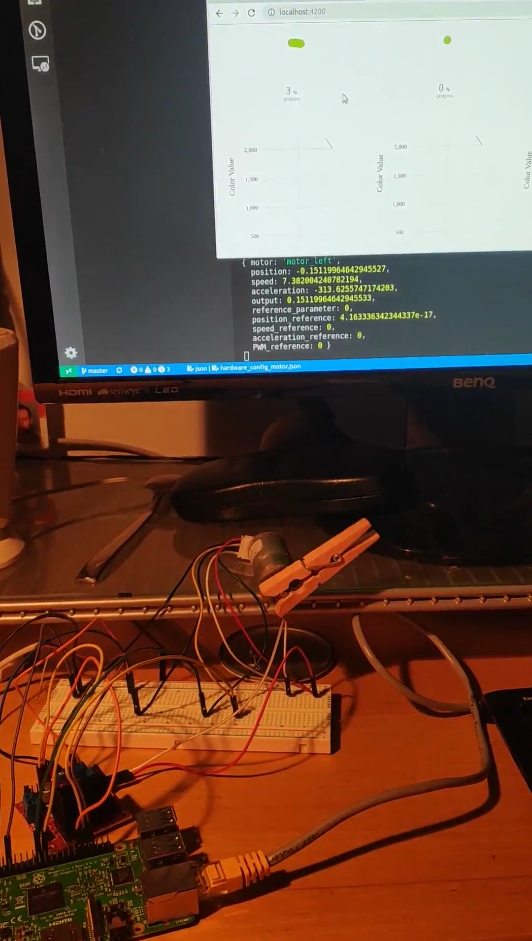
\includegraphics[width=7cm]{img/peg.png}
    \caption{Picture of the set up to control the peg.}
    \label{fig: control peg}
\end{figure}

Once knowing the constants that worked well for our peg,
we proceed the same method with the flywheel position but having a
starting point from the peg experiment.


\subsection{Speed control}
The input variable is the desired speed. We get the real speed by dividing the incremental angle
by the period (50 ms). This leaded to noisy measurements, so we decided to apply an average filter (3 samples) to
the result.

We use the motor speed control to be able to control the direction in which the robot is moving.
We transform a two-axis joystick signal (x,y) into speed set points for the PID of the wheels
 with the following formula:
\begin{equation}
    \begin{split}
    Speed_{right} = x + y \\
    Speed_{left} = x - y    
    \end{split}
\end{equation}
\subsection{Inclination control}
In order to control the inclination of the platform we also used a PID controller.
We sense the inclination of the platform with the accelerometer, and then we compute the error
as the difference between desired inclination and sensed inclination. Them, the we feed the 

\begin{itemize}
    \item In the flywheel case we simply output this error to the flywheel PWM motor signal.
    \item In the pendulum case this output is mapped to domain from -90 degrees to 90 degrees.
    Then this signal feeds another PID controller to control the position of the pendulum. We know
    the position of the pendulum by adding the inclination we sense to the rotation of the flywheel motor.
\end{itemize}
